{\large
\textbf{{\LARGE Week 8}}
\section{Neurale Netwerken}
\subsection{Lineaire neurale netwerken}
Lineaire netwerken zijn altijd terug te herleiden tot $Y=\beta X$. Zo is ook onderstaande neurale netwerk hiernaar terug te herleiden:
\[Y=\sum\limits_{j=1}^qv_j(\sum\limits_{i=0}^pu_{ij}X_i)=(\boldsymbol{U}\overrightarrow{v}) \overrightarrow{X}=\overrightarrow{\beta} \overrightarrow{X}\]
%---------------TikZ_______________
\tikzset{%
  every neuron/.style={
    circle,
    draw,
    minimum size=1cm
  },
  neuron missing/.style={
    draw=none, 
    scale=4,
    text height=0.333cm,
    execute at begin node=\color{black}$\vdots$
  },
}
\begin{center}
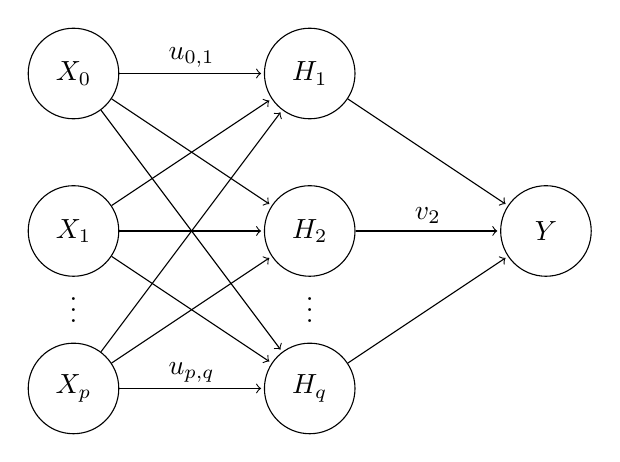
\begin{tikzpicture}[shorten >=1pt]
        \tikzstyle{unit}=[draw,shape=circle,minimum size=1.15cm]

        \node[unit](x0) at (0,4){$X_0$};
        \node at (1.5,4.2){$u_{0,1}$};
        \node[unit](x1) at (0,2){$X_1$};
        \node(dots) at (0,1.1){\vdots};
        \node[unit](xp) at (0,0){$X_p$};
        \node at (1.5,0.2){$u_{p,q}$};

        \node[unit](h1) at (3,4){$H_1$};
        \node[unit](h2) at (3,2){$H_2$};
        \node at (4.5,2.2){$v_{2}$};
        \node(dots) at (3,1.1){\vdots};
        \node[unit](hq) at (3,0){$H_q$};
        
        \node[unit](y) at (6,2){$Y$};
 
        \draw[->] (x0) -- (h1);
        \draw[->] (x0) -- (h2);
        \draw[->] (x0) -- (hq);

        \draw[->] (x1) -- (h1);
        \draw[->] (x1) -- (h2);
        \draw[->] (x1) -- (hq);

        \draw[->] (xp) -- (h1);
        \draw[->] (xp) -- (h2);
        \draw[->] (xp) -- (hq);
        
        \draw[->] (h1) -- (y);
        \draw[->] (h2) -- (y);
        \draw[->] (hq) -- (y);

    \end{tikzpicture}
\end{center}
%---------------TikZ_______________

\noindent Een opeenstapeling van lineaire transformaties blijft een lineaire transformatie. Om uit het lineaire regime te ontsnappen moeten we een niet-lineaire transformatie op iedere laag toepassen, de zogenoemde activatiefunctie.

\subsection{Logistische neurale netwerken (sigmoid)}
De sigmoid-activatiefunctie zal toegepast worden, waardoor de volgende formule en netwerk ontstaan:
\[Y=\sum\limits_{j=1}^qv_j\varphi(\sum\limits_{i=0}^pu_{ij}X_i)=(\textbf{U}\overrightarrow{v}) \overrightarrow{X}=\overrightarrow{\beta} \overrightarrow{X}\]

\begin{center}
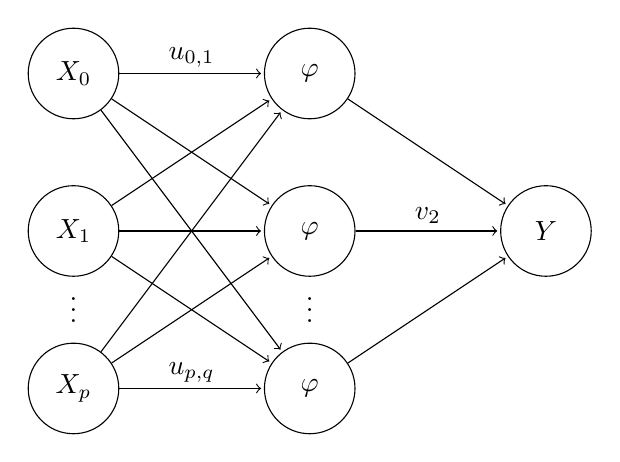
\begin{tikzpicture}[shorten >=1pt]
        \tikzstyle{unit}=[draw,shape=circle,minimum size=1.15cm]

        \node[unit](x0) at (0,4){$X_0$};
        \node at (1.5,4.2){$u_{0,1}$};
        \node[unit](x1) at (0,2){$X_1$};
        \node(dots) at (0,1.1){\vdots};
        \node[unit](xp) at (0,0){$X_p$};
        \node at (1.5,0.2){$u_{p,q}$};

        \node[unit](h1) at (3,4){$\varphi$};
        \node[unit](h2) at (3,2){$\varphi$};
        \node at (4.5,2.2){$v_{2}$};
        \node(dots) at (3,1.1){\vdots};
        \node[unit](hq) at (3,0){$\varphi$};
        
        \node[unit](y) at (6,2){$Y$};
 
        \draw[->] (x0) -- (h1);
        \draw[->] (x0) -- (h2);
        \draw[->] (x0) -- (hq);

        \draw[->] (x1) -- (h1);
        \draw[->] (x1) -- (h2);
        \draw[->] (x1) -- (hq);

        \draw[->] (xp) -- (h1);
        \draw[->] (xp) -- (h2);
        \draw[->] (xp) -- (hq);
        
        \draw[->] (h1) -- (y);
        \draw[->] (h2) -- (y);
        \draw[->] (hq) -- (y);

    \end{tikzpicture}
\end{center}

\noindent De structuur van het feed forward netwerk is:\\
\begin{minipage}{0.6\textwidth}
\begin{enumerate}
    \item Invloer \hfill $\overrightarrow{X}$
    \item Matrix vermenigvuldiging (weights) \hfill $\textbf{U}\overrightarrow{X}$
    \item niet-lin. transformatie (activatie) \hfill $\varphi (\textbf{U}\overrightarrow{X})$
    \item lin. combinatie \hfill $\overrightarrow{v}\varphi (\textbf{U}\overrightarrow{X})$
\end{enumerate}
\end{minipage}

\noindent Er kunnen ook meerdere lagen toegevoegd worden. Het is niet per definitie zo dat meer lagen voor een beter resultaat zorgen. Het aantal nodes is minstens net zo belangrijk. Voor meer informatie, zie \textit{Deep, Skinny Neural Networks are not Universal Approximators}.\\

\noindent
Twee nodes per laag kan mogelijk geen goede voorspelling maken, want er zitten maar twee grensvlakken aan verbonden als er maar twee nodes per layer aanwezig zijn. Zo kan er bijvoorbeeld geen cirkel gevormd worden bij 6, 2-dimensionale layers (a), terwijl dat met een enkele 3-node-layer wel gaat (b).
\begin{figure}[h]
    \centering
    \includegraphics[width=0.8\linewidth]{Images/layers probleem.png}
    \caption*{}
    \label{fig:layer}
\end{figure}\vspace{-1cm}

\subsection{Hoe trainen we een neuraal netwerk?}
Neem een netwerk met $l$ lagen, van groottes $n_1$ t/m $n_l$, activatiefunctie $\varphi^1$ t/m $\varphi^l$ en gewichten $\textbf{U}^1$ t/m $\textbf{U}^l$. Dus:
\[Y=g(\overrightarrow{X})=\varphi^l(\textbf{U}^l\varphi^{l-1}(\textbf{U}^{l-1}\dots\varphi^2(\textbf{U}^2\varphi(\textbf{U}\overrightarrow{X}))))\]
We introduceren een loss functie $L(\hat{y}),y$. 
\[L(\hat{y}),y=L(g(\overrightarrow{x}),y)\]

\noindent Het gewicht $u_{ij}^k$ is het gewicht dat hoort bij de pijl van de node $i$ in laag $k-1$ naar node $j$ in laag $k$. We kunnen met de kettingregel de loss differentiëren naar $u_{ij}^k$.
\[\frac{\partial L}{\partial u_{ij}^k}=L'\varphi^{l'}\textbf{U}^l\varphi^{l-1'}\dots \varphi^{k+1'}\textbf{U}^{k+1}\varphi_i^{k-1}\]
waar $\varphi_i^{k-1}$ de activatie van de $i^{de}$ neuron in laag $k-1$ is.\\

\noindent We zien dat de afgeleide alleen afhangt van:
\begin{itemize}
    \item de afgeleiden van de lagen rechts
    \item de activatie van de laag links
\end{itemize}
We kunnen dus redelijk efficiënt al deze afgeleiden van rechts naar links uitrekenen. Dit algoritme heet \textit{back propagation}. Dit wordt gebruikt in het volgende neurale netwerk cyclus:
\begin{enumerate}
    \item Bepalen van gewichten
    \item De loss functie bepalen met de feedforward fase
    \item Back propagation vanaf loss functie om gewichten te optimaliseren
    \item Repeat
\end{enumerate}

\subsection{Stochastic Gradient Descent}
\noindent Om onze gemiddelde loss $\bar{L}$ nu te minimaliseren gaan we als volgt te werk:
\begin{enumerate}
    \item We splitsen de data op in kleine random batches
    \item Voor iedere waarneming in een batch bepalen we $\frac{\partial L}{\partial u_{ij}^k}$
    \item Deze afgeleiden middelen we tot $\frac{\partial \bar{L}}{\partial u_{ij}^k}$
    \item We passen de gewichten als volgt aan:
    \[u_{ij}^k(t+1)=u_{ij}^k(t)-r\frac{\partial \bar{L}}{\partial u_{ij}^k}\]
    hier is $r$ de \textit{learning rate}.
    \item Als de volledige dataset op deze manier is doorlopen noemen we dit een epoch en herhalen we dit proces.
\end{enumerate}

\textbf{Batchsize}\\
Een te kleine batchsize kan zorgen voor slecht trainen van het model, omdat er dan van enkele klassen data in een batch kan zitten. Als het model enkel daarop traint, traint het niet op alle klassen (traint te specifiek). Een batchsize van 32 is meestal groot genoeg, representatief voor data. Bij veel klassen kies je voor een grotere batchsize. 

\subsection{Vanishing Gradient Problem}
\noindent Veel activatiefuncties vlakken af bij grote waardes van hun invoer. Hun afgeleides zijn dus heel klein en worden ook nog met elkaar vermenigvuldigd. Het gevolg is dat $u_{ij}^k$ voor kleine k nauwelijks aangepast word en dat het netwerk nauwelijks leert. Om dat probleem (deels) op te lossen wordt tegenwoordig vaak de ReLU-activatiefunctie gebruikt.
\begin{figure}[h]
    \centering
    \includegraphics[width=0.6\linewidth]{Images/vgp.png}
    \caption*{}
    \label{fig:layer}
\end{figure}

\newpage
\subsection{Voorbereiding}
Voorbereiding van het maken van een neuraal netwerk:
\begin{itemize}
    \item Probleemanalyse
    \item Data verzameling
    \item Train/test split
    \item Data verkenning
    \item Keuze loss-functie
    \item Keuze metrieken
\end{itemize}
\textbf{Feature selection}\\
Model kan slechter scoren als er betekenisloze variabelen in het model verwerkt zijn. Je wilt de variabelen afgaan en analyseren welke belangrijk zijn.\\

\textbf{Problemen met modelverbetering}
\begin{table}[h]
    \centering
    \begin{tabular}{|p{6cm}|p{5cm}|}
    \hline
    \textbf{Probleem} & \textbf{Oplossing}\\ \hline
         Trainen doet niks, je loss veranderd niet of nauwelijks per epoch en het model leert niks. & Learning rate of batchsize aanpassen. \\ \hline
         Het model traint wel, maar krijgt geen goede resultaten. Het verslaat simpele baselines niet of nauwelijks. Denk aan val\_acc die niet omhoog gaat. & Data probleem/model: (1) te weinig data, (2) misclassificatie, (3) verkeerde aanpak.\\\hline
         Het model traint en krijgt redelijke resultaten, maar na verloop van tijd gaat het nooit overfitten en blijft het dus underfit. Denk aan stagneren van train\_acc en val\_acc. & Meer lagen toevoegen/lagen groter maken.\\ \hline
         Duurt lang. & Geduld hebben. \\ \hline
    \end{tabular}
    \caption*{}
    \label{tab:my_label}
\end{table}

%plaatjes toevoegen

\textbf{Regularisatie}\\
Na het behalen van een goede loss-epoch-grafiek willen we het moment van overfitten zo lang mogelijk uitstellen. 
\begin{itemize}
    \item Early stopping (stoppen bij laagste val\_acc)
    \item Netwerk verkleinen als groot netwerk overfit, te klein blijft underfit. Probeer de juiste samenstelling te vinden)
    \item $L_1$ en/of $L_2$ regularisatie. (bij grote modellen werkt het niet goed)
    \item Dropout (willekeurige activaties op 0 zetten, bij grotere modellen werkt het wel goed)
\end{itemize}
\begin{figure}[h]
    \centering
    \includegraphics[width=0.8\linewidth]{Images/regularisaties.png}
    \caption*{}
    \label{fig:regularisatie}
\end{figure}
\begin{figure}[h!]
    \centering
    \includegraphics[width=0.8\linewidth]{Images/samenvattingNN.png}
    \caption*{}
    \label{fig:samenvatting}
\end{figure}
}
